\documentclass[11pt,letterpaper]{spie}

% Commonly used packages
\usepackage{natbib}
\usepackage{epsfig}
\usepackage{graphicx}
\usepackage{pgf}  
\usepackage{caption}
\usepackage{multirow}
\usepackage[normalem]{ulem}
\usepackage{color}
\usepackage{pdfpages}
\usepackage[breaklinks,colorlinks=true, pdfstartview=FitV, linkcolor=blue, 
            citecolor=blue, urlcolor=blue]{hyperref}
\usepackage{rotating}
\usepackage{url}
\usepackage{amsmath}
\usepackage{amssymb}
\usepackage{bm}

% Bibliography
%\bibliographystyle{apj_w_etal}
%\citestyle{aa}
%/Users/jaguirre/Documents/Latex/journals.tex
%\pagenumbering{arabic}
%\pagestyle{plain}

\thispagestyle{empty}
% ------------------- Title and Author -----------------------------
\title{The Mini Radio Telescope (MRT):\\
A Tool for Education and Outreach}
%\author{James Aguirre}

\begin{document}

\maketitle

The Mini Radio Telescope funded by this grant is designed to be a portable demonstration and teaching tool.  This year it was was demonstrated at Boys' Latin High School, used in Prof. Aguirre's ASTR250 course at Penn, used as part of the Experimental Physics Research Academy summer program for high school students at Penn, and used in public demonstrations at the Philadelphia Science Festival both in Clark Park and on Philadelphia Parkway.

\begin{figure}[h]
\centering
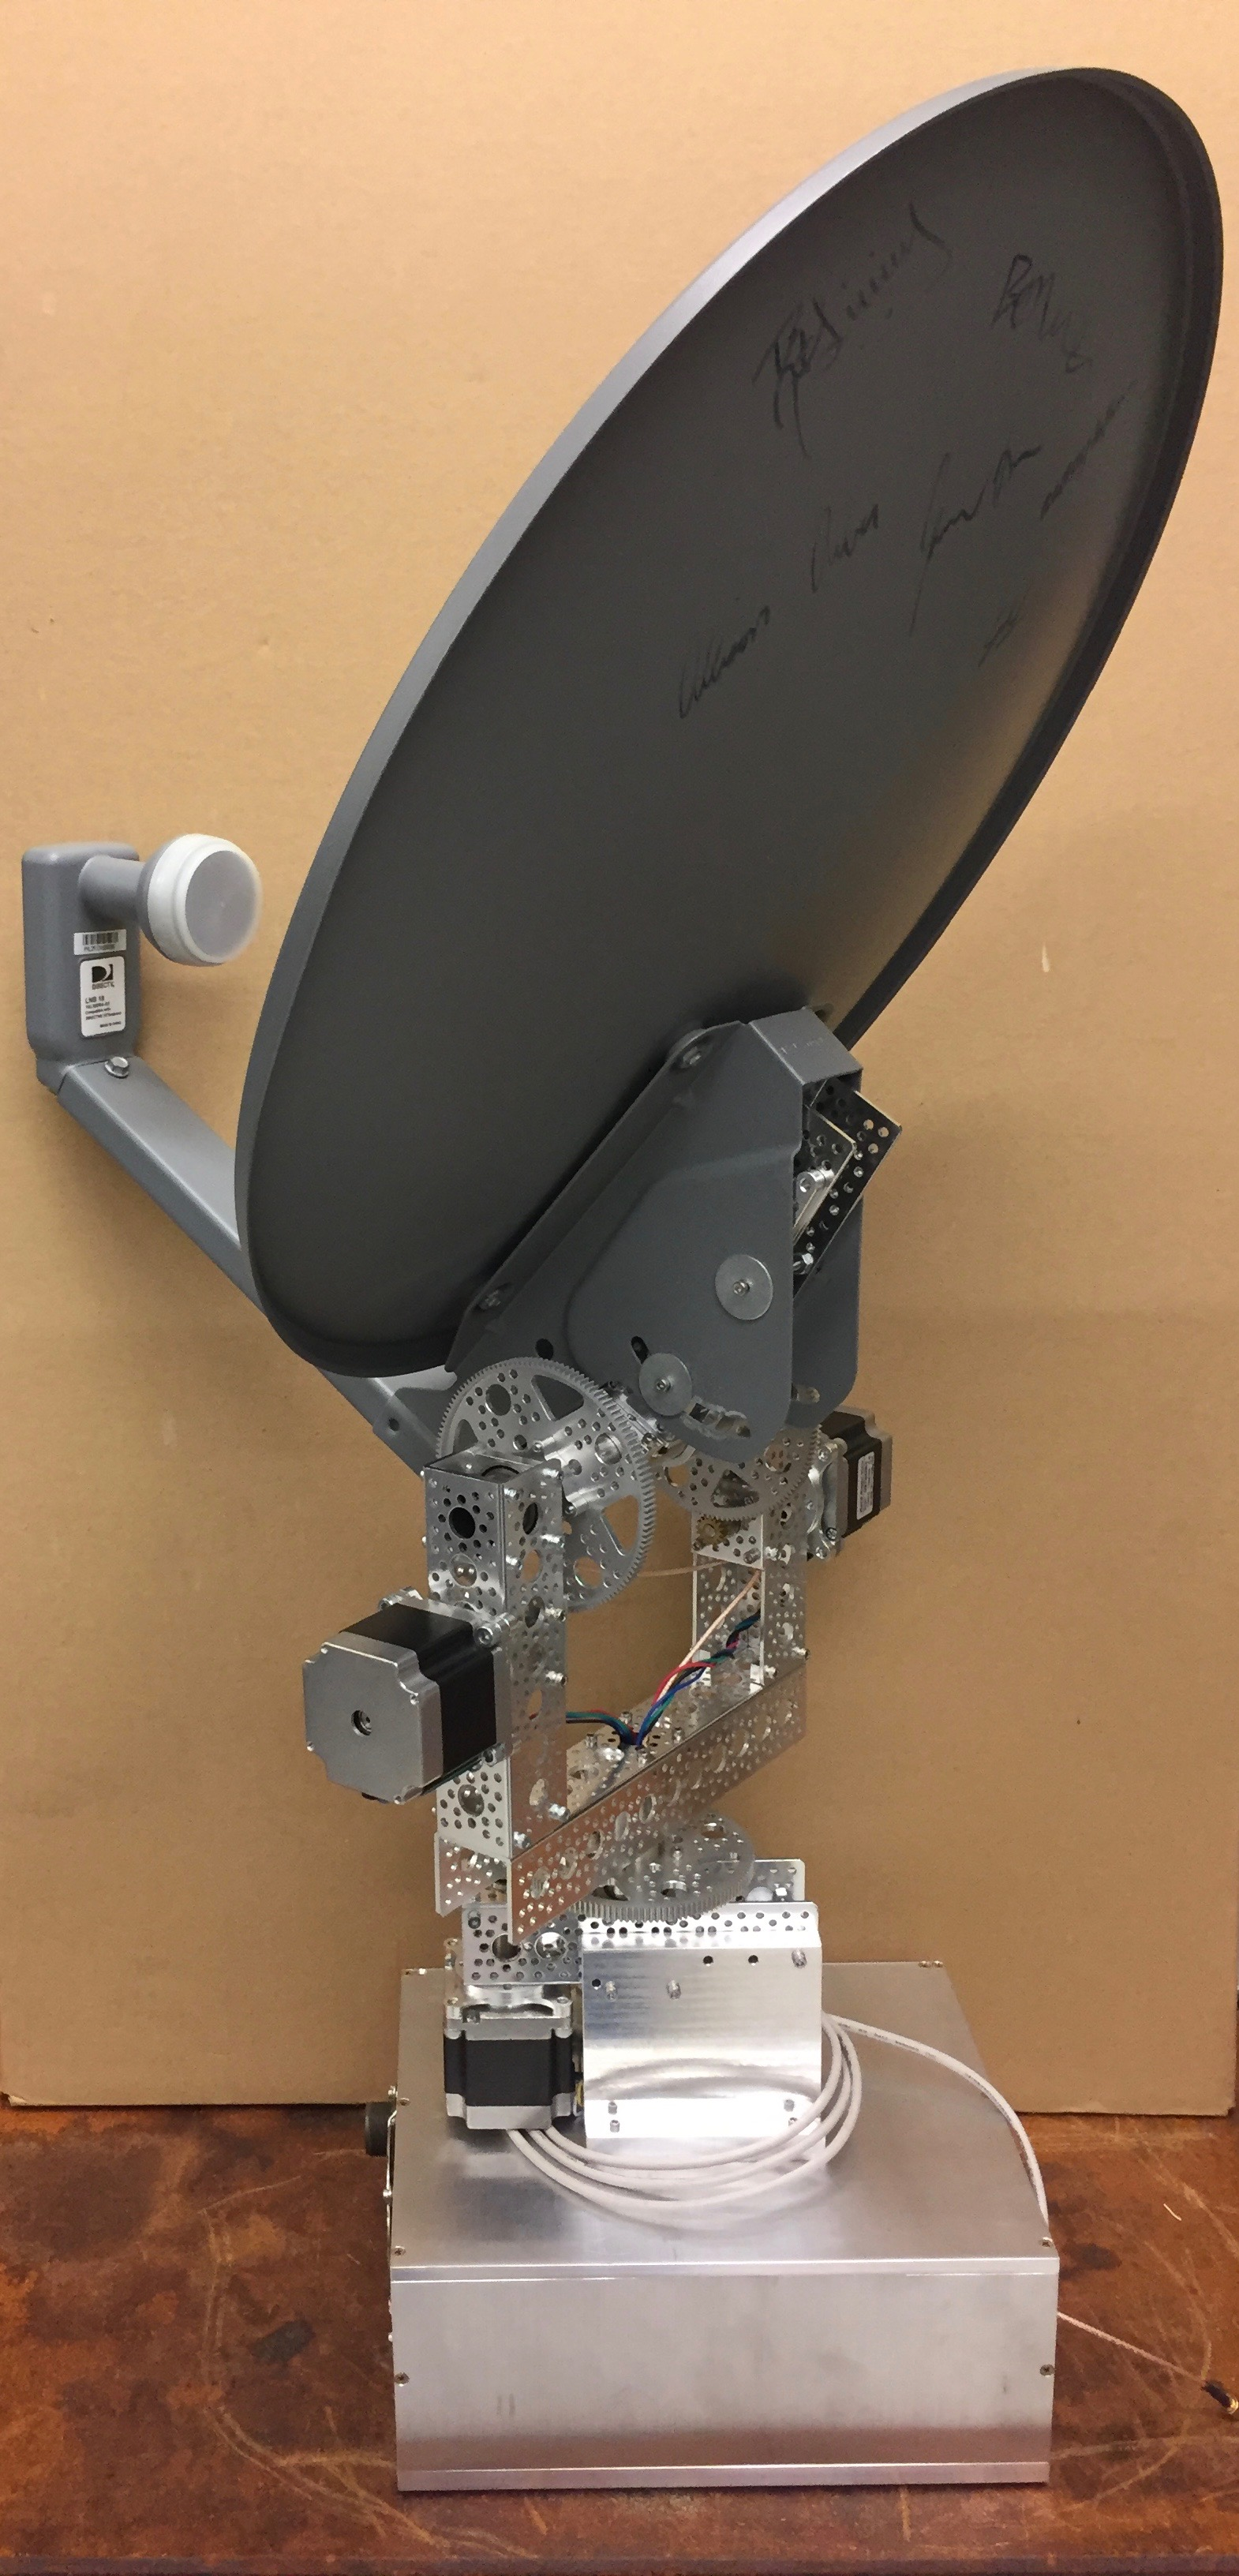
\includegraphics[height=6in]{new_box.jpeg}
\vspace{5pt}
\caption{The current mechanical design from hobby electronics components (Actobotics) was simple and quick, but insufficiently rigid.
}
\label{fig:Devices}
\end{figure}


\begin{figure}[h]
\centering
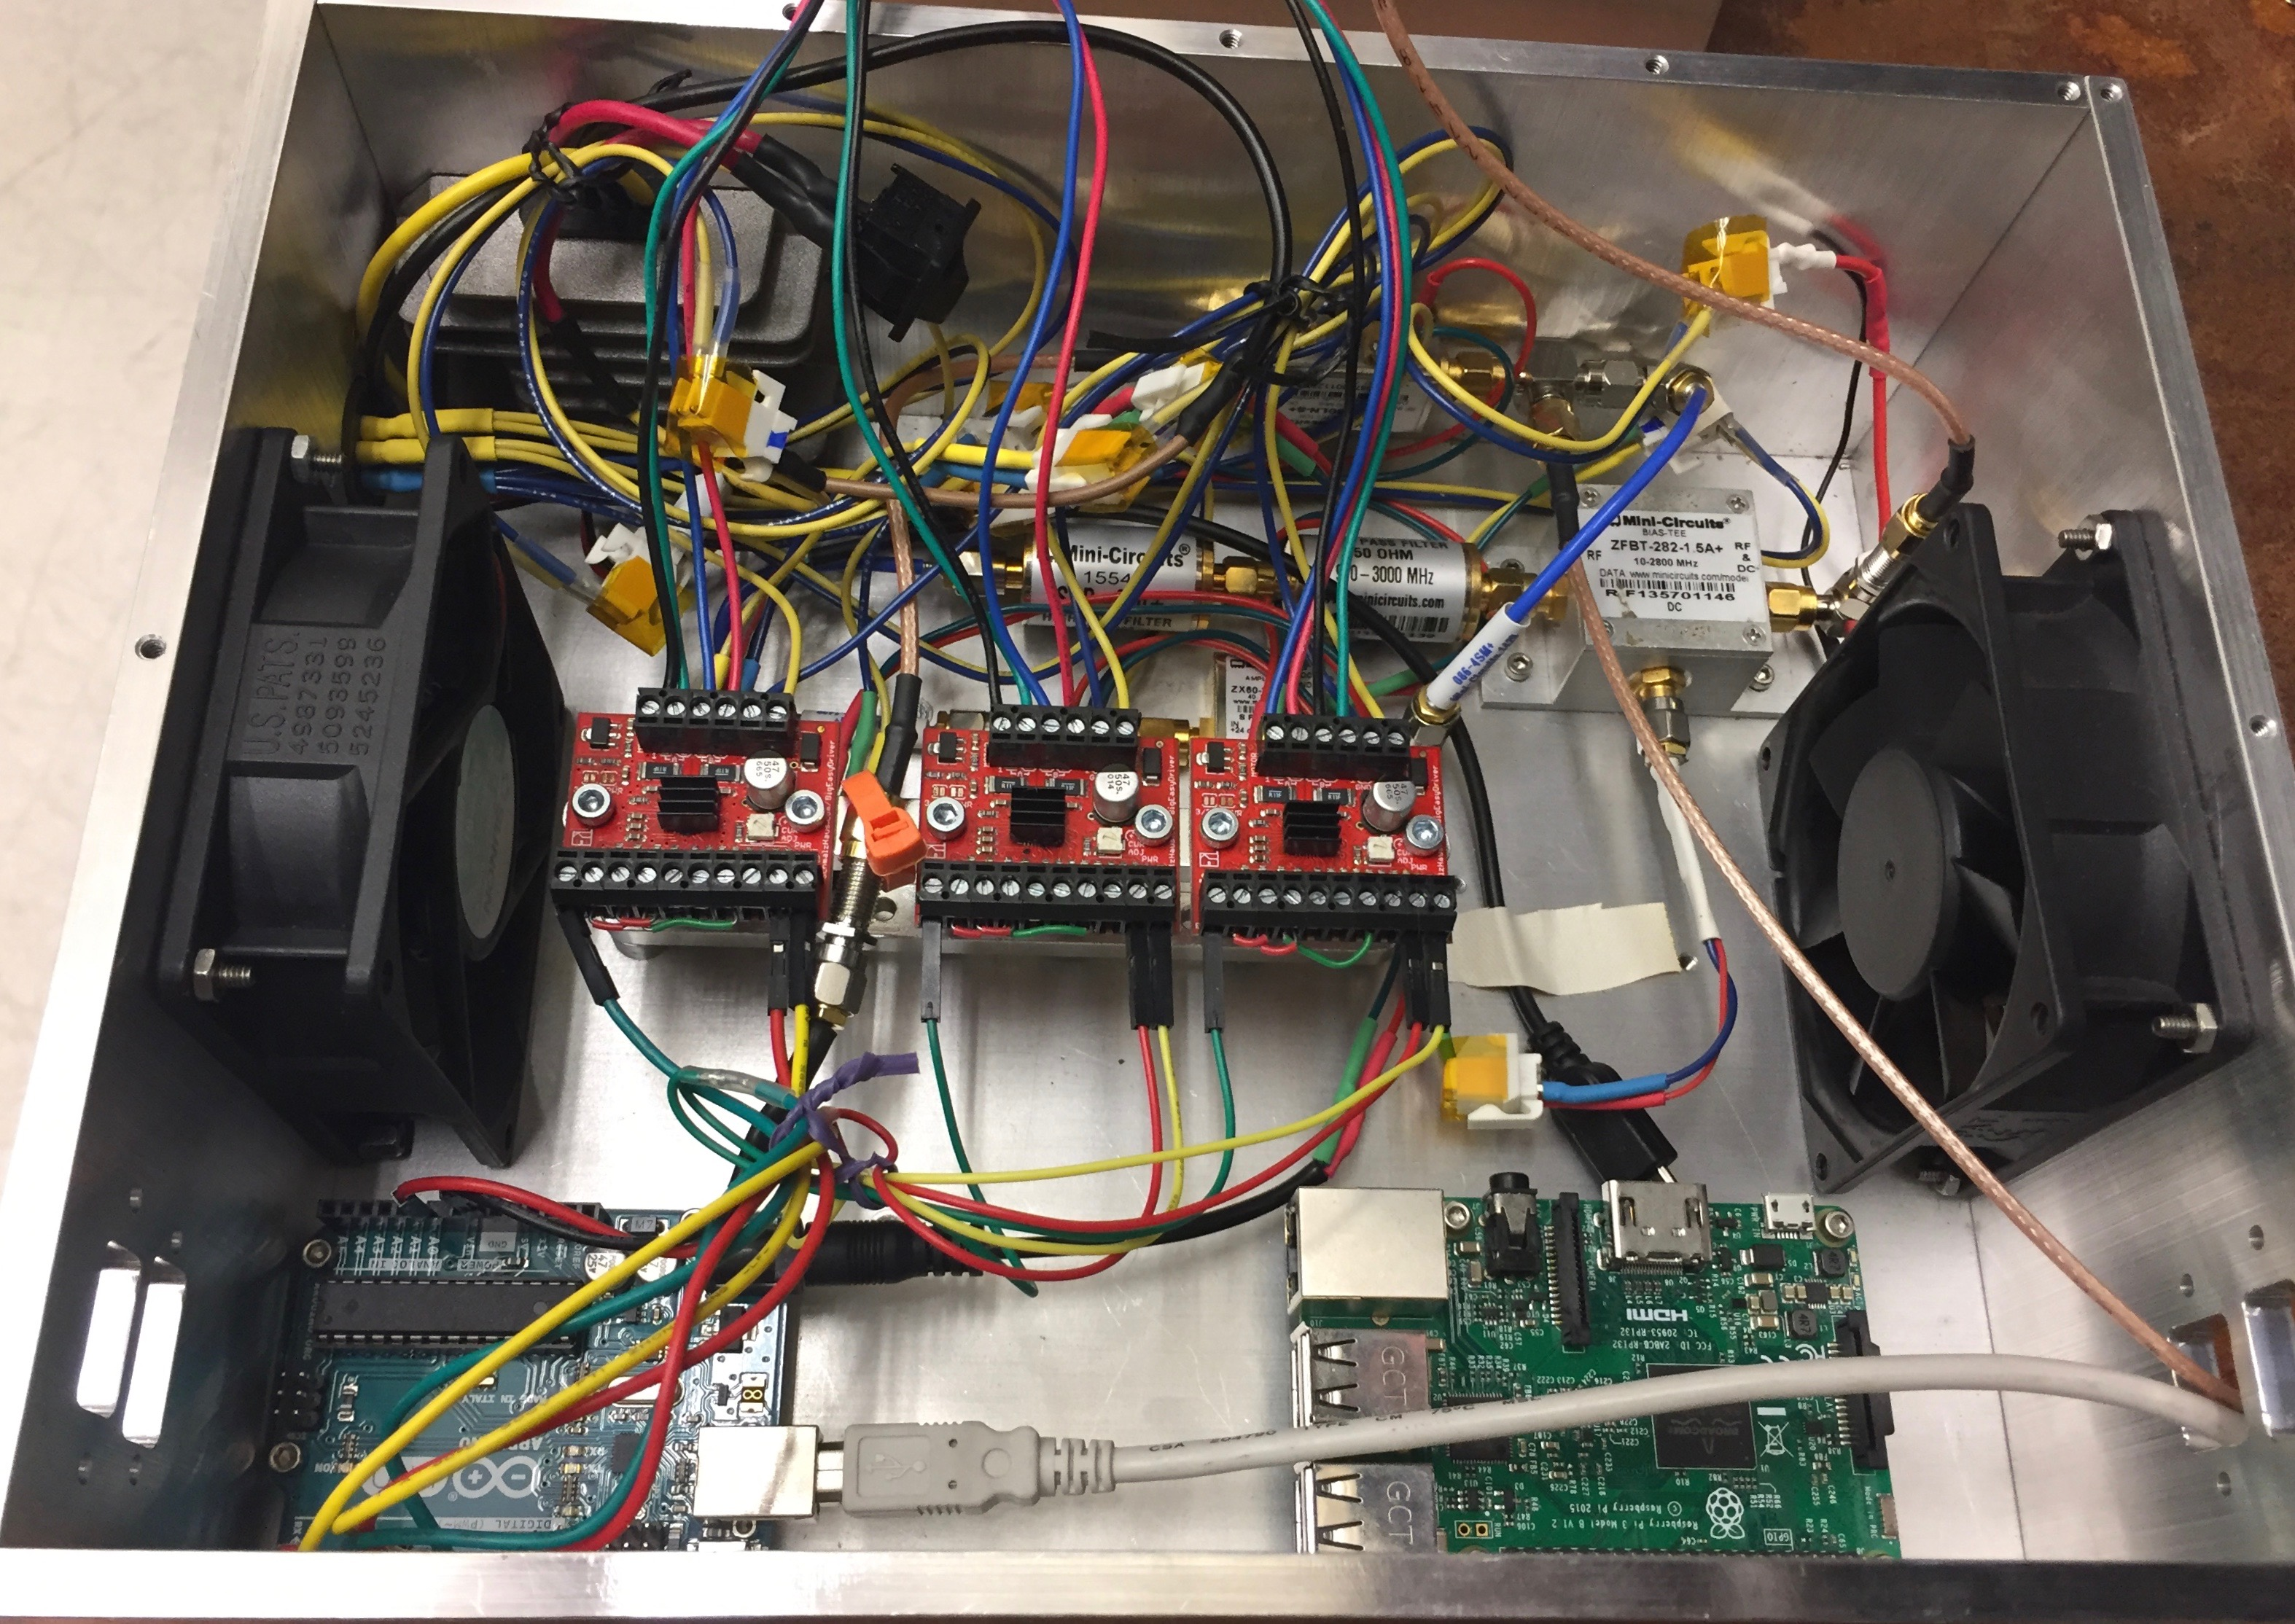
\includegraphics[width=6in]{new_electronics.jpeg}
\vspace{5pt}
\caption{The new electronics are housed in an enclosure designed to be more rugged.
}
\label{fig:Devices}
\end{figure}


\begin{figure}[h]
\centering
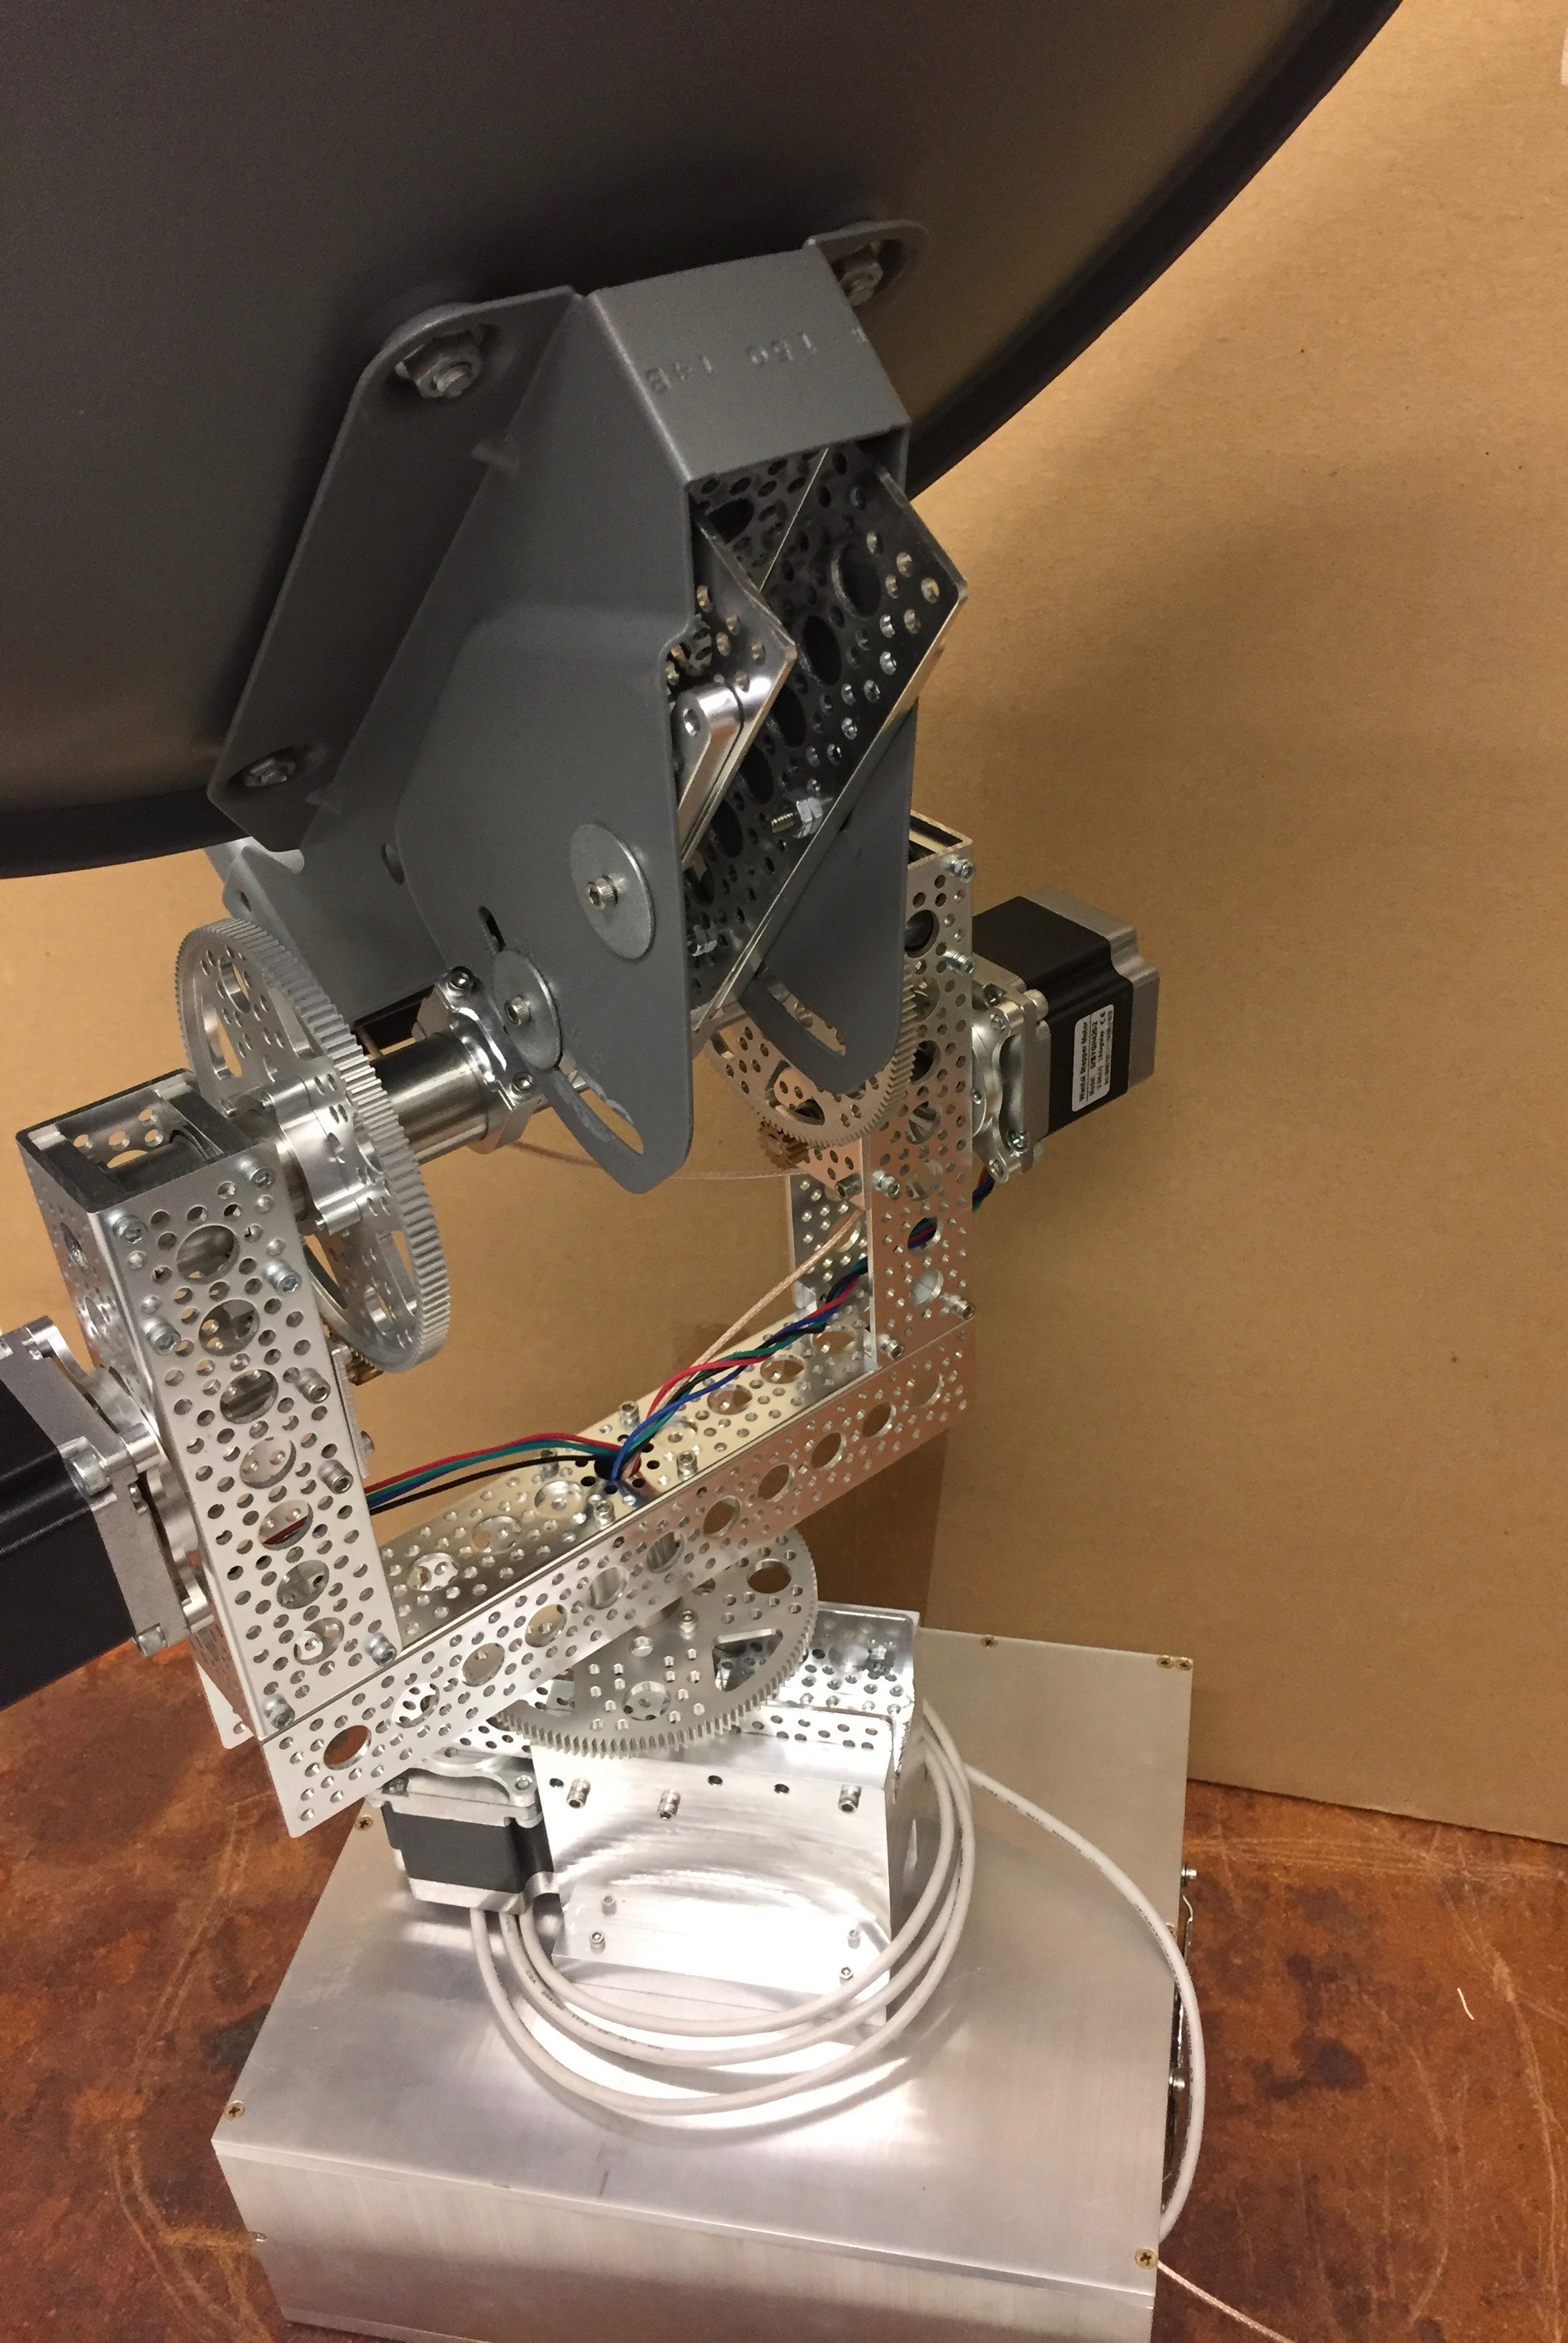
\includegraphics[height=6in]{new_closeup.jpeg}
\vspace{5pt}
\caption{The current mechanical design from hobby electronics components (Actobotics) was simple and quick, but insufficiently rigid.
}
\label{fig:Devices}
\end{figure}



\begin{figure}[h]
\centering
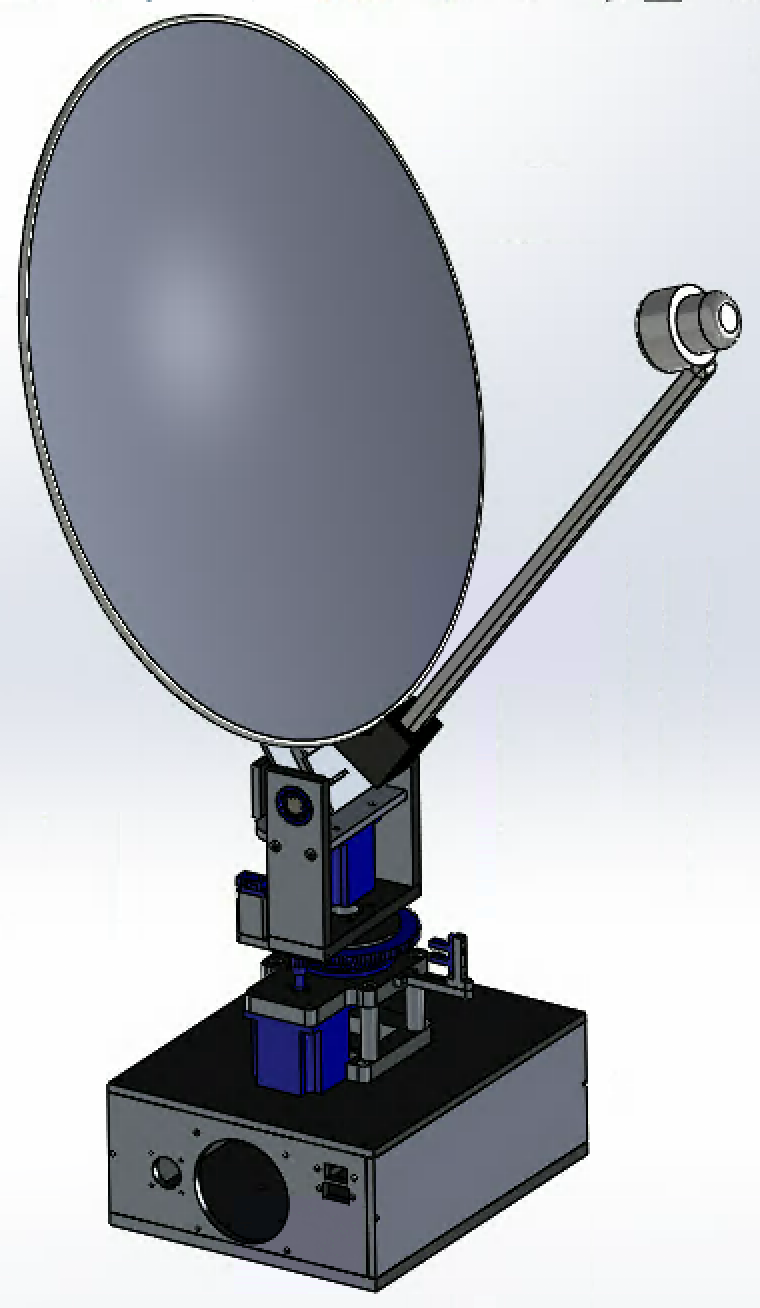
\includegraphics[height=6in]{NewMRT/threequarter.png}
\vspace{5pt}
\caption{The new simplified MRT telescope mount design.}
\label{fig:NewMRTthreequarter}
\end{figure}

\begin{figure}[h]
\centering
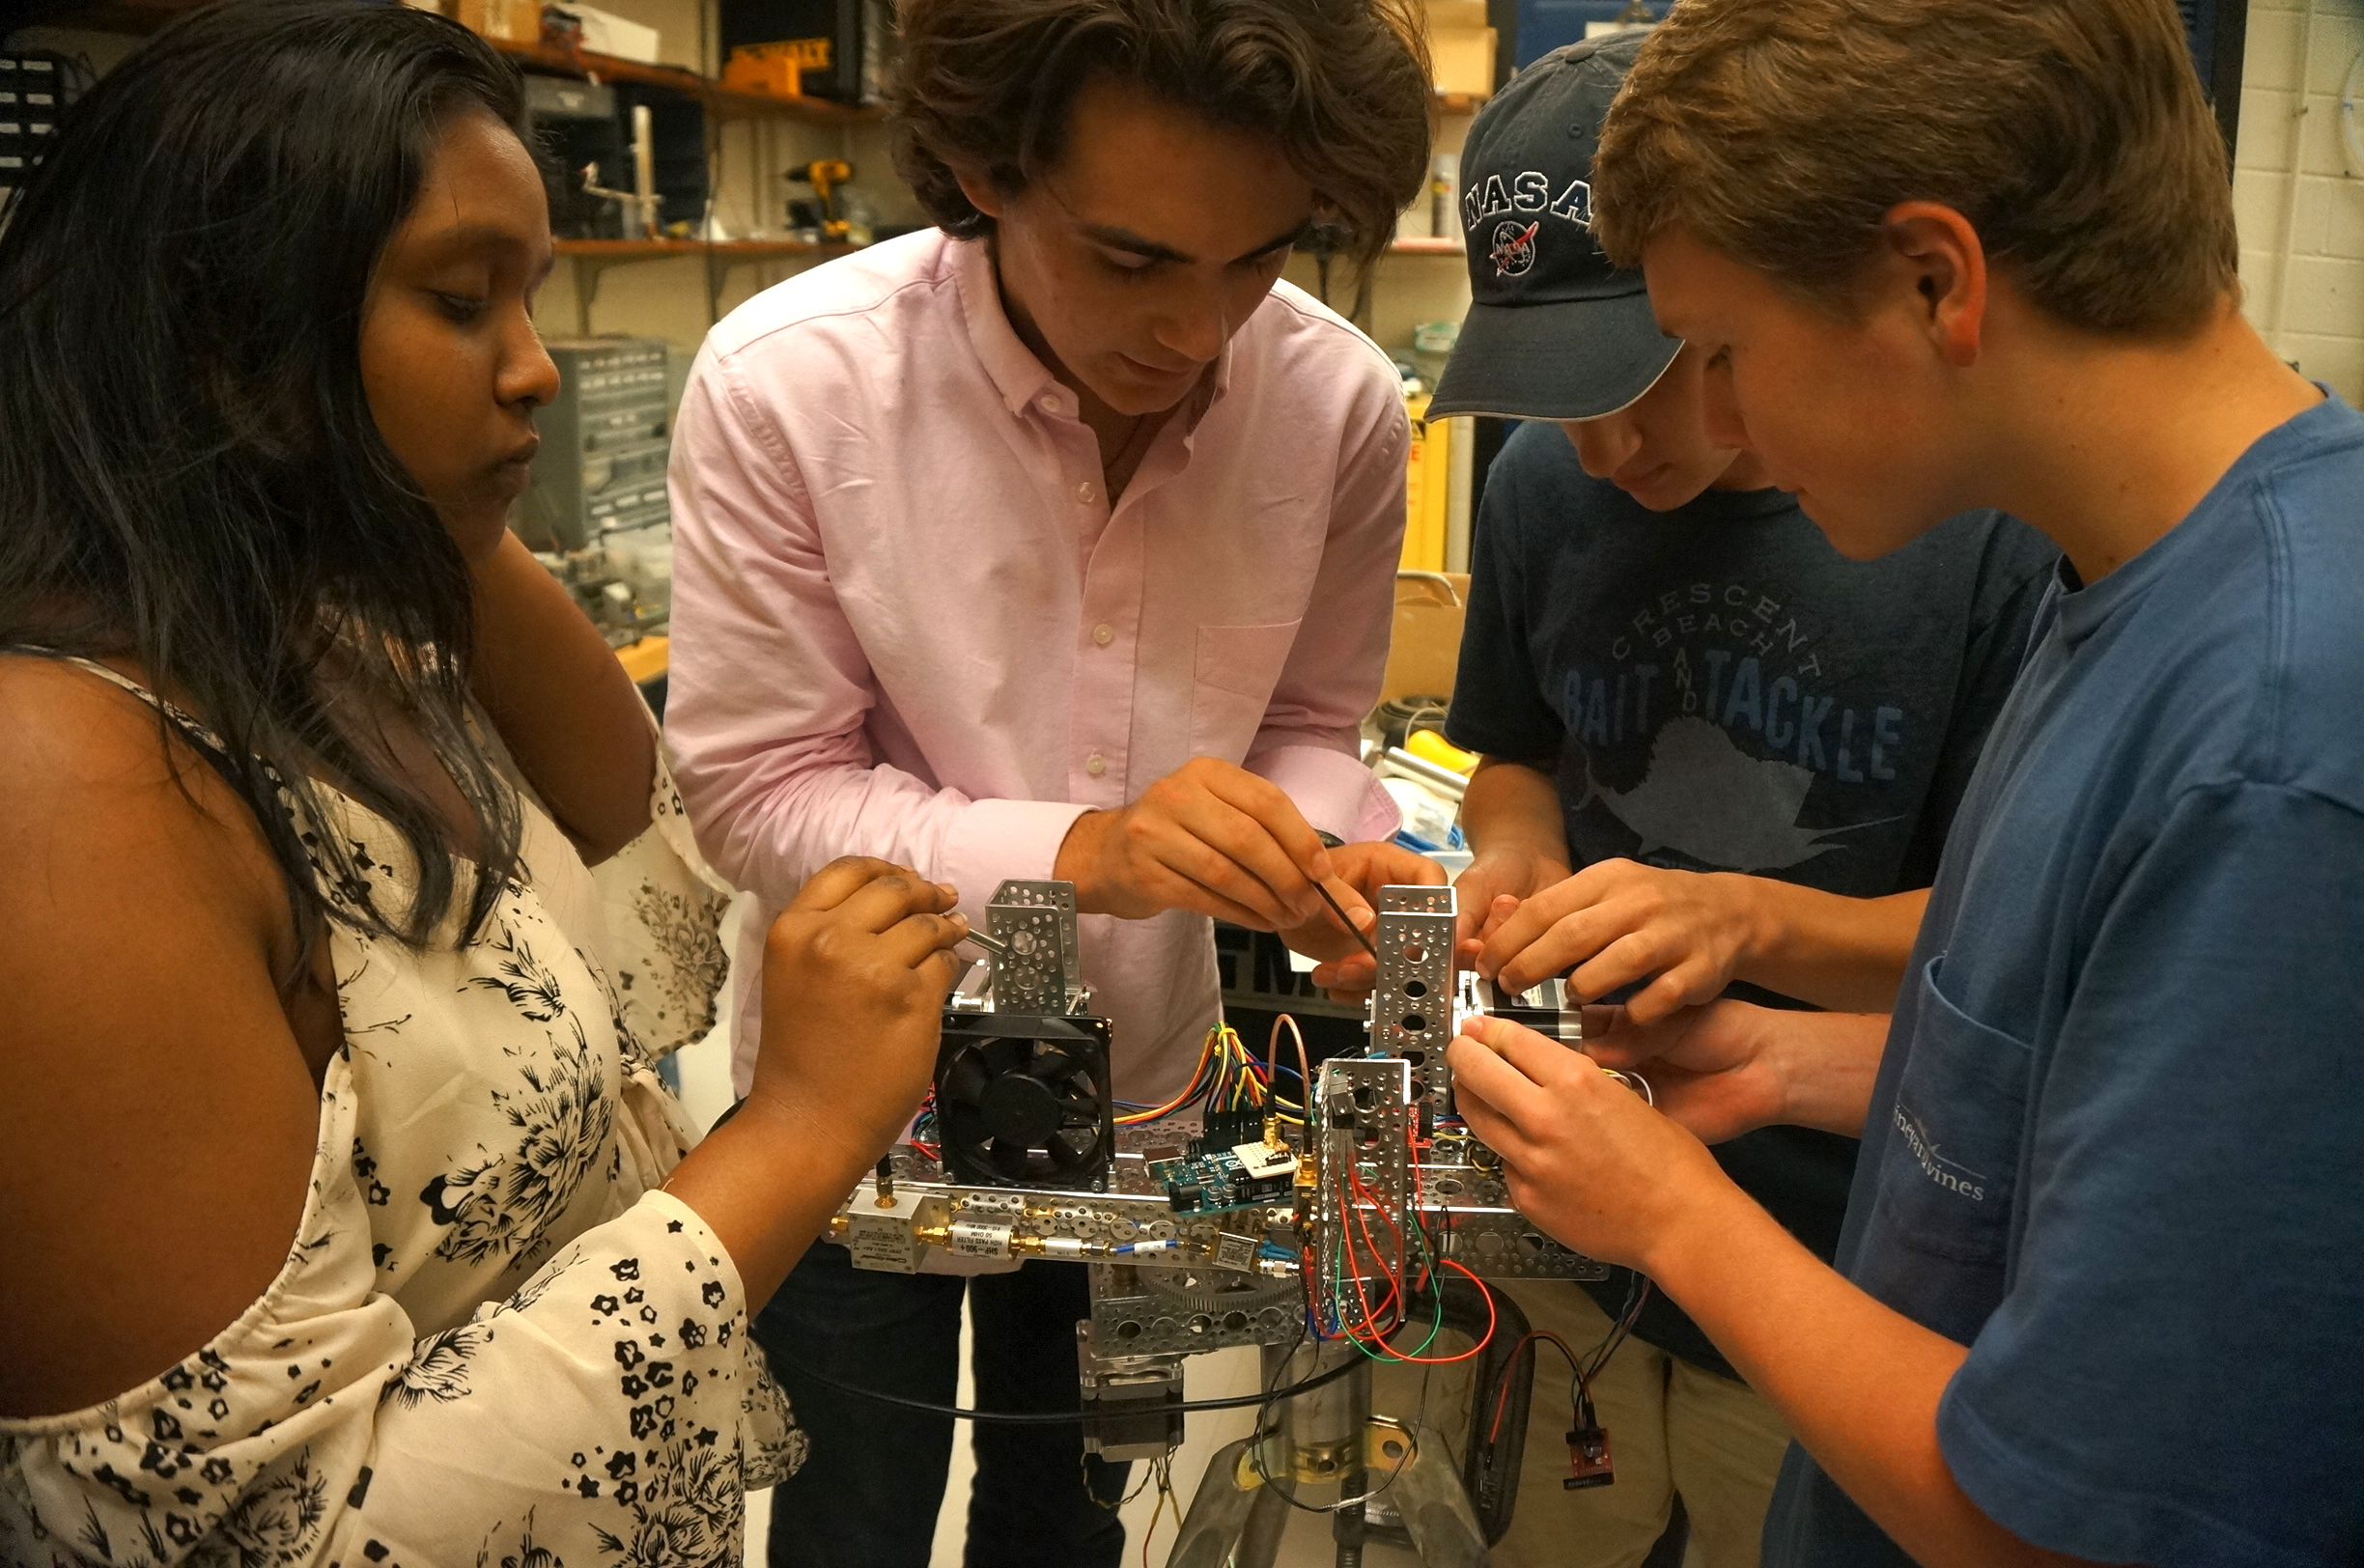
\includegraphics[width=6.5in]{EPRA_working.jpg}
\vspace{5pt}
\caption{EPRA students working on the MRT, summer 2017.}
\label{fig:Devices}
\end{figure}

\begin{figure}[h]
\centering
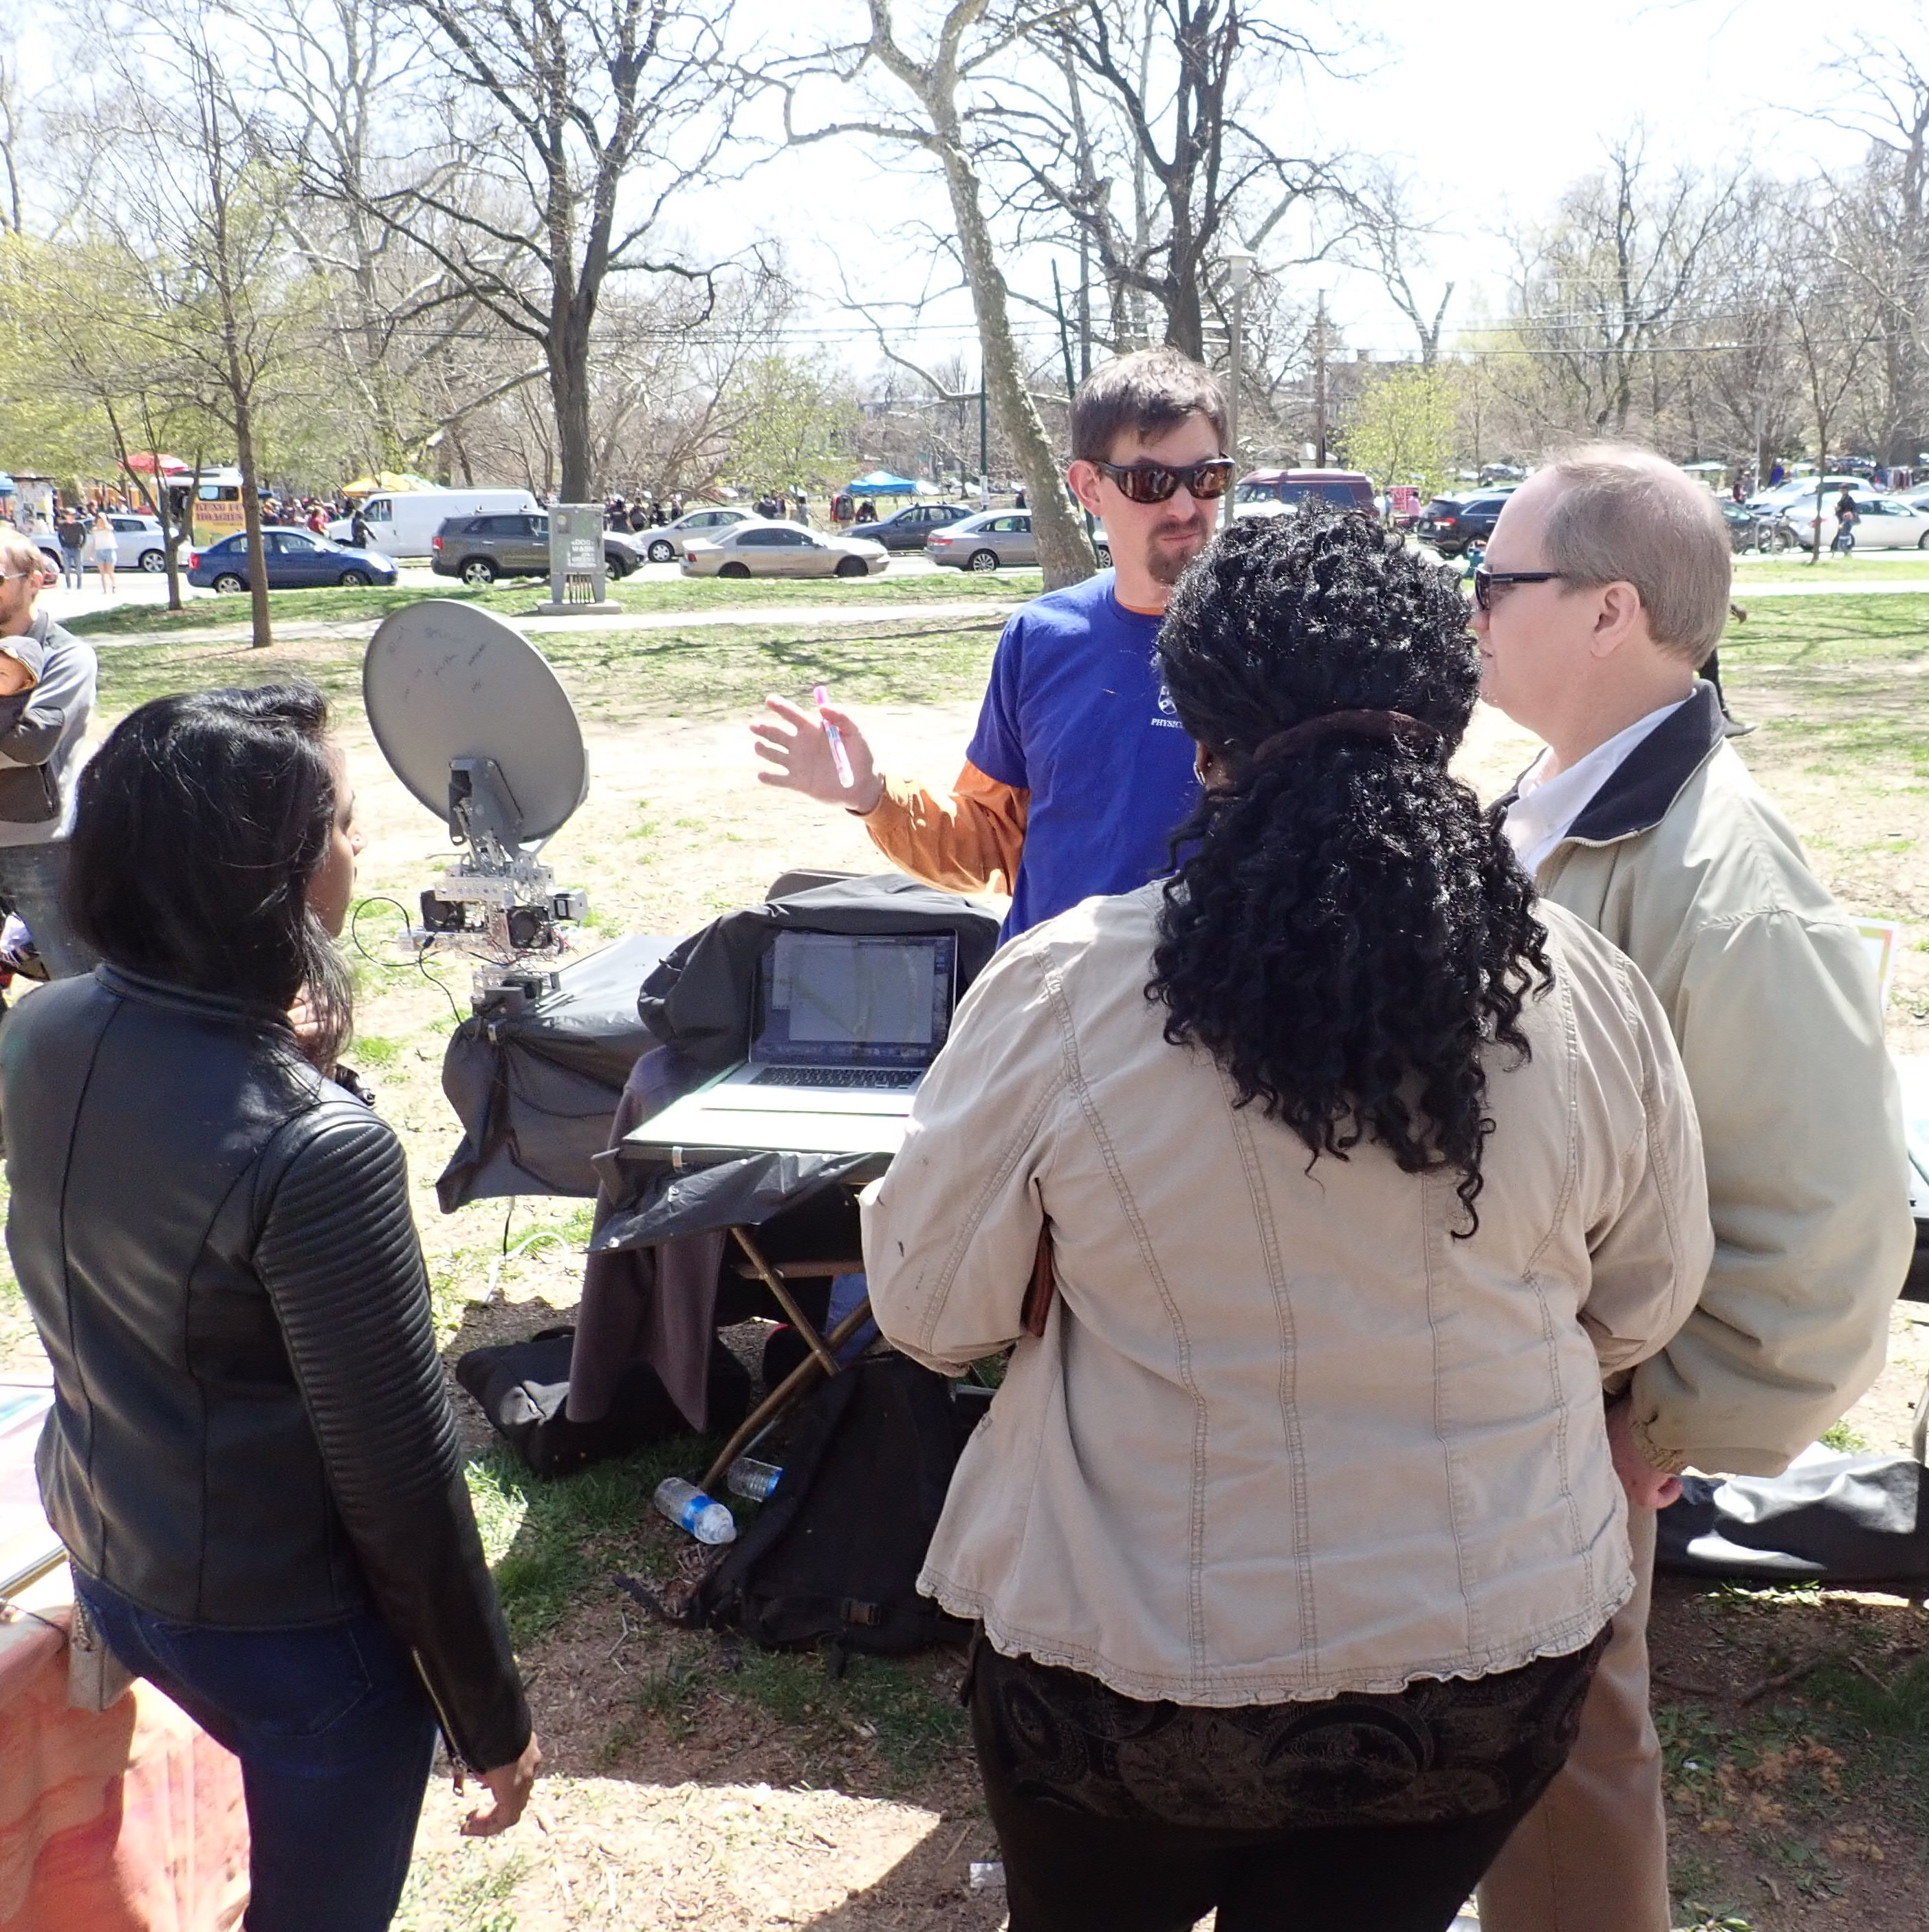
\includegraphics[width=6.5in]{ClarkPark.jpg}
\vspace{5pt}
\caption{Prof.~Aguirre with the MRT in Clark Park as part of the Philadelphia Science Festival, 21 April 2018.}
\label{fig:ClarkPark}
\end{figure}

\begin{figure}[h]
\centering
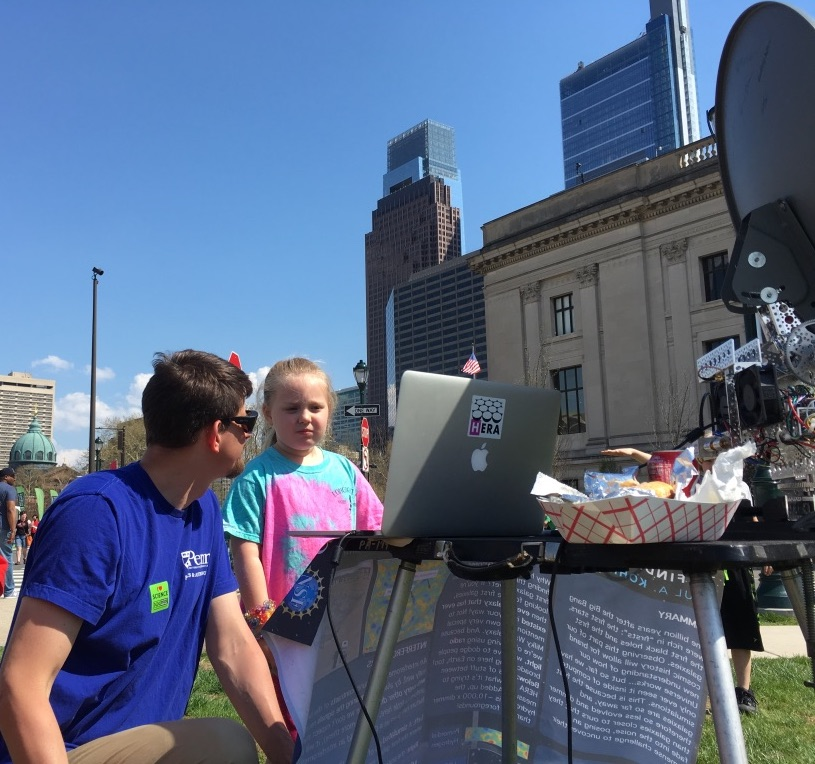
\includegraphics[width=6.5in]{PSFCarnival2.jpg}
\vspace{5pt}
\caption{Explaining the telescope to a young visitor to the Philadelphia Science Festival's Carnival, 28 April 2018.}
\label{fig:Devices}
\end{figure}

\end{document}


